% PASUPASASTRA — Manual Pengguna. Build: latexmk -xelatex manual.tex
\documentclass[11pt,a4paper,oneside]{report}
\usepackage{fontspec}
\setmainfont{DejaVu Sans}[Scale=0.92]
\setmonofont{DejaVu Sans Mono}[Scale=0.82]
\usepackage[a4paper,margin=2.3cm,headheight=15pt]{geometry}
\usepackage[table]{xcolor}
\usepackage{graphicx,booktabs,tabularx,longtable,array,enumitem,titlesec,fancyhdr,listings,tikz,pgfplots}
\usepackage[most]{tcolorbox}
\usepackage[hidelinks]{hyperref}
\usetikzlibrary{arrows.meta,positioning,fit,calc}
\pgfplotsset{compat=1.18}
\hyphenpenalty=10000
\exhyphenpenalty=10000
\sloppy

\definecolor{navy}{HTML}{0E1624}
\definecolor{ink}{HTML}{14213D}
\definecolor{body}{HTML}{4A5568}
\definecolor{teal}{HTML}{0F6E77}
\definecolor{cyan}{HTML}{39D0D8}
\definecolor{warn}{HTML}{B45309}
\definecolor{danger}{HTML}{B42318}
\definecolor{paper}{HTML}{F3F4EF}
\definecolor{demo}{HTML}{7C5CD6}

\titleformat{\chapter}[display]{\color{ink}\bfseries\Huge}{\color{teal}\large BAB \thechapter}{4pt}{}[\vspace{2pt}{\color{cyan}\rule{3cm}{3pt}}]
\titlespacing*{\chapter}{0pt}{0pt}{18pt}
\titleformat{\section}{\color{ink}\bfseries\Large}{\color{teal}\thesection}{8pt}{}
\titleformat{\subsection}{\color{ink}\bfseries\large}{\color{teal}\thesubsection}{8pt}{}
\setlist{itemsep=2pt,topsep=4pt}
\setlength{\parskip}{5pt}
\setlength{\parindent}{0pt}

\pagestyle{fancy}\fancyhf{}
\fancyhead[L]{\small\color{body}PASUPASASTRA · Manual Pengguna}
\fancyhead[R]{\small\color{body}\leftmark}
\fancyfoot[C]{\small\color{body}\thepage}
\renewcommand{\headrulewidth}{0.3pt}
\fancypagestyle{plain}{\fancyhf{}\fancyfoot[C]{\small\color{body}\thepage}\renewcommand{\headrulewidth}{0pt}}

\lstset{basicstyle=\ttfamily\small,backgroundcolor=\color{paper},frame=single,rulecolor=\color{paper!80!black},
  breaklines=true,breakatwhitespace=false,columns=flexible,keepspaces=true,postbreak=\mbox{\textcolor{teal}{$\hookrightarrow$}\space},showstringspaces=false,xleftmargin=4pt,xrightmargin=4pt,
  aboveskip=6pt,belowskip=6pt,literate={→}{{$\rightarrow$}}1 {–}{{--}}1}
\newcommand{\code}[1]{\texttt{\small #1}}
\newcommand{\ui}[1]{\textbf{\color{ink}#1}}

\newtcolorbox{catatan}[1][Catatan]{colback=teal!6,colframe=teal,fonttitle=\bfseries,title=#1,boxrule=0.6pt,arc=2pt}
\newtcolorbox{peringatan}[1][Peringatan keselamatan]{colback=warn!7,colframe=warn,fonttitle=\bfseries,title=#1,boxrule=0.6pt,arc=2pt}
\newtcolorbox{bahaya}[1][Bahaya]{colback=danger!6,colframe=danger,fonttitle=\bfseries,title=#1,boxrule=0.8pt,arc=2pt}

\renewcommand{\chaptername}{Bab}
\renewcommand{\contentsname}{Daftar Isi}
\renewcommand{\appendixname}{Lampiran}
\renewcommand{\figurename}{Gambar}
\renewcommand{\tablename}{Tabel}
\begin{document}
\begin{titlepage}
\pagecolor{navy}\color{white}
\vspace*{3cm}
{\color{cyan}\rule{4cm}{5pt}}\par\vspace{1cm}
{\large\color{cyan} MANUAL PENGGUNA DAN PENERAPAN}\par\vspace{0.6cm}
{\fontsize{46}{50}\selectfont\bfseries PASUPASASTRA}\par\vspace{0.4cm}
{\LARGE Unified Command Center For Multi-drone Operations}\par\vspace{2cm}
{\large Ground Control Station multi-drone: konsol operator, server, bridge DJI dan Autel, video, dan analitik AI}\par
\vfill
{\color{cyan!60!white}\large Versi perangkat lunak 0.3.0 \quad·\quad DarmawanWeb / nextgen-gcs}\par
{\color{cyan!60!white} Dokumen internal. Isi dapat berubah mengikuti pengembangan.}
\end{titlepage}
\pagecolor{white}\color{black}
\tableofcontents
\chapter{Pendahuluan}
PASUPASASTRA adalah \emph{ground control station} (GCS) untuk operasi banyak drone dari vendor berbeda dalam satu konsol. Operator melihat posisi dan status seluruh armada di satu peta, menonton video dari drone, ponsel, dan CCTV, menjalankan deteksi objek dan analisis adegan berbasis AI, serta mengirim perintah terbang dan misi waypoint ke drone yang mendukungnya.

Seluruh antarmuka operator berbahasa Indonesia. Seluruh sistem berjalan di server lokal (misalnya Mac Mini M4 di pos komando) tanpa layanan cloud wajib.

\section{Komponen}

\noindent\begin{tabularx}{\linewidth}{@{}>{\bfseries}l X@{}}
\toprule
Komponen & Fungsi \\ \midrule
Konsol (\code{fe/}) & Aplikasi operator Next.js, berjalan di browser dan sebagai aplikasi desktop Tauri. \\
\code{gcs-api} (\code{be/}) & Server FastAPI: autentikasi, registri drone dan kamera, endpoint bridge, perintah dan misi, simulator drone demo, perekaman penerbangan, tanya-jawab visual (VLM), speech-to-text. \\
\code{gcs-worker} (\code{be/}) & Proses inferensi: beberapa model YOLO per stream, hitungan grup, caption Moondream, video beranotasi. \\
MediaMTX & Server media: menerima RTMP/RTSP/SRT dan menyajikan WebRTC/HLS. \\
NATS & Bus pesan antara API dan worker. \\
PostgreSQL + TimescaleDB & Penyimpanan data, kejadian, audit, dan jejak terbang. \\
Ollama & Model bahasa-visual lokal (Moondream, penerjemah). \\
Bridge DJI (\code{bridges/\allowbreak{}dji-\allowbreak{}matrice-\allowbreak{}4t/}) & Aplikasi Android di remote DJI untuk Matrice 4T (MSDK v5.17). \\
Bridge Autel (\code{bridges/\allowbreak{}autel-\allowbreak{}evo2-\allowbreak{}v3/}) & Aplikasi Android di Smart Controller V3 untuk EVO II V3 (Autel SDK v1.5). \\
\bottomrule
\end{tabularx}

Kode sumber ada di organisasi GitHub \code{DarmawanWeb}. Repositori utama \code{Pasupasastra} (infrastruktur dan dokumen) memuat konsol \code{pasupasastra-\allowbreak{}gcs-\allowbreak{}fe}, server \code{pasupasastra-\allowbreak{}gcs-\allowbreak{}be}, dan \code{PasupasastraBridge} sebagai \emph{submodule}. \code{PasupasastraBridge} memuat satu submodule per model drone: \code{pasupasastra-\allowbreak{}bridge-\allowbreak{}dji-\allowbreak{}matrice-\allowbreak{}4t} dan \code{pasupasastra-\allowbreak{}bridge-\allowbreak{}autel-\allowbreak{}evo2-\allowbreak{}v3}.

\section{Istilah}
\begin{description}[leftmargin=3.2cm,style=nextline]
\item[Bridge] Aplikasi di remote controller yang meneruskan telemetri ke server dan menjalankan perintah dari server.
\item[Interlock] Saklar \ui{Izinkan kendali dari GCS} di aplikasi bridge. Selama mati, drone hanya mengirim telemetri dan semua perintah ditolak.
\item[Drone demo] Wahana simulasi di server, berwarna ungu dengan label DEMO, untuk mendemonstrasikan fitur (termasuk drop payload) tanpa drone fisik.
\item[Stream] Satu sumber video: kamera drone atau kamera tetap (CCTV/ponsel).
\item[Kunci model] Nama pendek unik model deteksi, dipakai pada hitungan \code{model:kelas}.
\end{description}

\section{Status dokumen}
Manual ini menggambarkan versi 0.3.0. Bagian yang belum diuji di perangkat keras nyata ditandai jelas. Hasil pengujian otomatis dan pengukuran performa ada di Bab~\ref{bab:performa}.

\chapter{Arsitektur}
\begin{center}
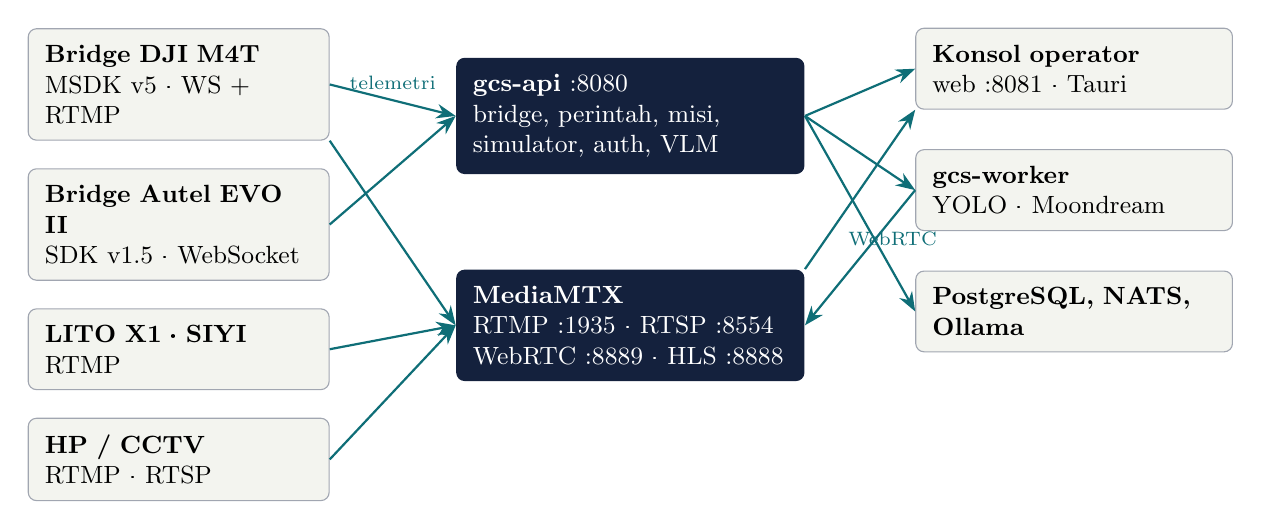
\begin{tikzpicture}[font=\small,
  box/.style={draw=ink!40,fill=paper,rounded corners=3pt,align=left,inner sep=6pt,text width=#1},
  dark/.style={fill=ink,text=white,rounded corners=3pt,align=left,inner sep=6pt,text width=#1},
  arr/.style={-{Stealth[length=7pt]},thick,teal}]
\node[box=3.4cm] (dji) {\textbf{Bridge DJI M4T}\\MSDK v5 · WS + RTMP};
\node[box=3.4cm,below=0.35cm of dji] (autel) {\textbf{Bridge Autel EVO II}\\SDK v1.5 · WebSocket};
\node[box=3.4cm,below=0.35cm of autel] (lito) {\textbf{LITO X1 · SIYI}\\RTMP};
\node[box=3.4cm,below=0.35cm of lito] (cctv) {\textbf{HP / CCTV}\\RTMP · RTSP};
\node[dark=4cm,right=1.6cm of dji,yshift=-0.4cm] (api) {\textbf{gcs-api} :8080\\bridge, perintah, misi,\\simulator, auth, VLM};
\node[dark=4cm,below=1.2cm of api] (mtx) {\textbf{MediaMTX}\\RTMP :1935 · RTSP :8554\\WebRTC :8889 · HLS :8888};
\node[box=3.6cm,right=1.4cm of api,yshift=0.6cm] (ui) {\textbf{Konsol operator}\\web :8081 · Tauri};
\node[box=3.6cm,below=0.5cm of ui] (worker) {\textbf{gcs-worker}\\YOLO · Moondream};
\node[box=3.6cm,below=0.5cm of worker] (db) {\textbf{PostgreSQL, NATS,}\\\textbf{Ollama}};
\draw[arr] (dji.east) -- node[above,font=\scriptsize]{telemetri} (api.west);
\draw[arr] (autel.east) -- (api.west);
\draw[arr] (dji.south east) -- (mtx.west);
\draw[arr] (lito.east) -- (mtx.west);
\draw[arr] (cctv.east) -- (mtx.west);
\draw[arr] (api.east) -- (ui.west);
\draw[arr] (api.east) -- (worker.west);
\draw[arr] (worker.west) -- (mtx.east);
\draw[arr] (api.east) -- (db.west);
\draw[arr] (mtx.north east) -- node[pos=0.3,below right,font=\scriptsize]{WebRTC} (ui.south west);
\end{tikzpicture}
\end{center}

\section{Alur data}
\begin{enumerate}
\item \textbf{Telemetri.} Bridge membuka WebSocket ke \code{gcs-api}. API menormalkan format vendor ke satu model telemetri, mendeteksi lepas landas dan mendarat, mencatat jejak terbang, lalu menyiarkan ke konsol melalui \code{/ws/realtime} dengan laju 5~Hz per drone.
\item \textbf{Perintah.} Konsol memanggil \code{POST /\allowbreak{}drones/\allowbreak{}\{id\}/\allowbreak{}commands}. API memeriksa izin, kapabilitas bridge, dan batas keselamatan, lalu mengirim permintaan ke bridge dan menunggu \emph{ack}. Semua perintah dicatat di log audit.
\item \textbf{Video.} Drone dan ponsel mengirim RTMP ke MediaMTX. Kamera IP (RTSP/HLS) ditarik oleh MediaMTX ke jalur \code{src/<id>}. Konsol menonton lewat WebRTC (WHEP).
\item \textbf{AI.} API mengirim \emph{desired state} ke worker lewat NATS. Worker membaca RTSP, menjalankan model, menerbitkan deteksi dan caption, dan mempublikasikan video beranotasi ke jalur \code{ai/<path>}.
\end{enumerate}

\section{Port jaringan}

\noindent\begin{tabularx}{\linewidth}{@{}l l X@{}}
\toprule
Port & Protokol & Kegunaan \\ \midrule
8080 & HTTP/WS & API, WebSocket realtime, endpoint bridge \\
8081 & HTTP & Konsol web + proxy API (Caddy) \\
1935 & TCP & RTMP masuk dari drone, ponsel, CCTV \\
8554 & TCP & RTSP (worker membaca dan menerbitkan) \\
8889 & HTTP & WebRTC WHEP untuk konsol \\
8189 & UDP & Media WebRTC \\
8888 & HTTP & HLS \\
8890 & UDP & SRT masuk \\
\bottomrule
\end{tabularx}


\chapter{Penerapan server}
\section{Kebutuhan}
\begin{itemize}
\item Mac Mini M4 (disarankan RAM 16~GB atau lebih) dengan macOS terbaru, IP LAN tetap (contoh di manual: \code{192.168.1.10}).
\item Docker Desktop, Homebrew, Node.js 20+, Python 3.12, Ollama, PM2.
\item Router Wi-Fi yang menghubungkan server dengan remote controller drone dan laptop operator.
\end{itemize}

\section{Instalasi satu kali}
\begin{lstlisting}
git clone <repo> pasupasastra && cd pasupasastra
# ffmpeg, venv Python, ollama pull moondream + llama3.2:3b, pm2
./infra/scripts/setup-mac.sh
cd infra && cp .env.example .env
\end{lstlisting}
Isi \code{.env} minimal:

\noindent\begin{tabularx}{\linewidth}{@{}l X@{}}
\toprule
Variabel & Isi \\ \midrule
\code{LAN\_IP} & IP LAN server, dipakai sebagai kandidat WebRTC. \\
\code{PUBLIC\_\allowbreak{}WEBRTC\_\allowbreak{}URL} & \code{http:\allowbreak{}/\allowbreak{}/\allowbreak{}<LAN\_\allowbreak{}IP>:\allowbreak{}8889} \\
\code{POSTGRES\_\allowbreak{}PASSWORD} & Kata sandi database, acak. \\
\code{GCS\_\allowbreak{}JWT\_\allowbreak{}SECRET} & String acak panjang (minimal 32 karakter). \\
\code{GCS\_\allowbreak{}ADMIN\_\allowbreak{}PASSWORD} & Kata sandi awal akun \code{admin}; ganti setelah login pertama. \\
\code{GCS\_\allowbreak{}BRIDGE\_\allowbreak{}TOKEN} & Opsional. Jika diisi, URL bridge wajib memakai \code{?token=...}. \\
\bottomrule
\end{tabularx}

\section{Build konsol}
\begin{lstlisting}
cd app && npm ci
NEXT_PUBLIC_API_URL=http://192.168.1.10:8081/api npm run build   # hasil di app/out
\end{lstlisting}
Tanpa \code{NEXT\_\allowbreak{}PUBLIC\_\allowbreak{}API\_\allowbreak{}URL}, konsol berjalan dalam \emph{mode simulasi} penuh di browser tanpa server; berguna untuk pelatihan dan demo.

Aplikasi desktop: \code{npm run tauri build} dengan variabel yang sama menghasilkan installer macOS/Windows.

\section{Menjalankan}
\begin{lstlisting}
cd infra
docker compose up -d --build          # MediaMTX, TimescaleDB, NATS, API, web
pm2 start pm2/ecosystem.config.cjs    # worker AI native (CoreML / VideoToolbox)
pm2 save && pm2 startup
\end{lstlisting}
Periksa kesehatan: \code{curl http:\allowbreak{}/\allowbreak{}/\allowbreak{}localhost:\allowbreak{}8080/\allowbreak{}health} harus berisi \code{"ok": true}, dan \code{"worker"} tidak \code{null} setelah worker berjalan.

Buka konsol di \code{http:\allowbreak{}/\allowbreak{}/\allowbreak{}192.\allowbreak{}168.\allowbreak{}1.\allowbreak{}10:\allowbreak{}8081}, masuk sebagai \code{admin}, lalu ganti kata sandi di \ui{Pengaturan → Akun}.

\section{Akun operator}
Tidak ada pendaftaran mandiri. Administrator membuat akun lewat CLI:
\begin{lstlisting}
docker compose exec api gcs-admin create-user \
    --username op1 --display-name "Operator 1" --role operator
docker compose exec api gcs-admin set-password --username op1
\end{lstlisting}
Peran: \code{admin} (semua), \code{operator} (mengubah data dan mengirim perintah), \code{observer} (hanya melihat).

\section{Server Linux dengan GPU NVIDIA}
\code{docker compose --profile gpu up -d} menjalankan worker CUDA dan Ollama di container. Model CoreML (\code{.mlpackage}) hanya berjalan pada worker macOS.

\section{Akses jarak jauh}
\begin{catatan}
Cloudflare Tunnel (\code{infra/\allowbreak{}cloudflared/\allowbreak{}config.\allowbreak{}example.\allowbreak{}yml}) hanya meneruskan HTTP: konsol, API, dan WebSocket berfungsi, tetapi media WebRTC (UDP) tidak. Untuk video langsung dari luar LAN gunakan VPN (WireGuard atau Tailscale) ke jaringan pos komando.
\end{catatan}

\section{Pemeliharaan}
\begin{itemize}
\item Cadangan database: \code{docker compose exec postgres pg\_\allowbreak{}dump -U gcs gcs > backup.\allowbreak{}sql}
\item Pembaruan: \code{git pull}, build ulang konsol, \code{docker compose up -d --build}, \code{pm2 restart gcs-worker}. Migrasi database berjalan otomatis saat API mulai.
\item Log: \code{docker compose logs -f api}, \code{pm2 logs gcs-worker}.
\end{itemize}

\chapter{Bridge drone}
Bridge adalah aplikasi Flutter + Kotlin di remote controller. Folder \code{bridges/dji} dan \code{bridges/autel} berisi \code{lib/} (UI Flutter) dan \code{android/} (kode native dan SDK). Gabungkan ke proyek Flutter masing-masing (yang memiliki \code{pubspec.yaml}) atau buat proyek baru dengan \code{flutter create} lalu salin kedua folder tersebut.

\section{Protokol singkat}
Bridge membuka WebSocket ke server, mengirim \code{hello} berisi kapabilitas, lalu telemetri berkala. Server mengirim \code{command} atau \code{mission} dengan \code{id}, bridge menjawab \code{ack} dengan \code{id} yang sama. Detail JSON ada di Lampiran~\ref{lamp:protokol}.

Kapabilitas \code{commands} dan \code{mission} hanya diumumkan bila interlock menyala. Konsol menonaktifkan tombol yang tidak didukung dan menampilkan alasannya.

\section{Batas keselamatan}
Dicek dua kali, di server dan di bridge (bridge memakai posisi GPS terbaru):
\begin{center}
\begin{tabular}{@{}l r@{}}
\toprule
Batas & Nilai \\ \midrule
Ketinggian titik misi & 5--120 m (dan tidak melebihi \emph{Ketinggian maks.} drone) \\
Jarak titik dari posisi drone & maks. 1000 m \\
Kecepatan & maks. 10 m/s \\
Jumlah titik & maks. 99 \\
\bottomrule
\end{tabular}
\end{center}

\section{Bridge DJI Matrice 4T}
\subsection{Prasyarat}
\begin{itemize}
\item Remote controller M4T yang didukung DJI Mobile SDK v5.17 (periksa daftar perangkat yang didukung di dokumentasi MSDK).
\item App key dari \code{developer.\allowbreak{}dji.\allowbreak{}com} untuk paket \code{com.\allowbreak{}darmawan.\allowbreak{}dronebridge}.
\item Android Studio, Flutter SDK, JDK 17.
\end{itemize}
\subsection{Build}
\begin{lstlisting}
cd bridges/dji/android
cp local.properties.example local.properties    # isi sdk.dir, flutter.sdk, DJI_API_KEY
cd .. && flutter build apk --release
adb install -r build/app/outputs/flutter-apk/app-release.apk
\end{lstlisting}
\begin{catatan}[Kunci API]
Kunci DJI dibaca dari \code{local.\allowbreak{}properties} (tidak di-commit) dan disisipkan ke manifest saat build. Jangan menulis kunci langsung di \code{AndroidManifest.\allowbreak{}xml}.
\end{catatan}
\subsection{Konfigurasi di aplikasi}

\noindent\begin{tabularx}{\linewidth}{@{}l X@{}}
\toprule
Isian & Nilai \\ \midrule
WebSocket URL & \code{ws:\allowbreak{}/\allowbreak{}/\allowbreak{}192.\allowbreak{}168.\allowbreak{}1.\allowbreak{}10:\allowbreak{}8080/\allowbreak{}telemetry/\allowbreak{}m4t-001} (akhir URL = ID drone di konsol) \\
RTMP URL & \code{rtmp:\allowbreak{}/\allowbreak{}/\allowbreak{}192.\allowbreak{}168.\allowbreak{}1.\allowbreak{}10:\allowbreak{}1935/\allowbreak{}m4t} \\
Izinkan kendali dari GCS & Mati untuk telemetri saja; nyalakan hanya saat pilot siap mengambil alih. Berlaku saat bridge dimulai. \\
\bottomrule
\end{tabularx}

Tekan \ui{START BRIDGE}. Bridge berjalan sebagai \emph{foreground service} dan tetap hidup saat aplikasi diminimalkan.

\subsection{Perilaku perintah (MSDK v5)}

\noindent\begin{tabularx}{\linewidth}{@{}l X@{}}
\toprule
Perintah & Implementasi dan catatan \\ \midrule
Aktifkan/matikan motor & \textbf{Tidak didukung terpisah} oleh MSDK v5. Motor menyala saat lepas landas dan mati otomatis setelah mendarat; bridge menjawab dengan penjelasan. \\
Lepas landas & \code{KeyStartTakeoff}: naik sekitar 1,2 m lalu hover. \\
Mendarat & \code{KeyStartAutoLanding}. \\
Kembali ke home & \code{KeyStartGoHome}. \\
Tahan posisi & Menjeda misi, atau \code{KeyStopGoHome} / \code{KeyStopAutoLanding}. \\
Terbang ke titik & Misi satu titik (KMZ), berakhir hover. \\
Misi waypoint & KMZ WPML dibuat di aplikasi, diunggah dengan \code{pushKMZFileToAircraft}, dijalankan dengan \code{startMission}. Ketinggian relatif titik lepas landas; hilang sinyal RC: kembali. \\
Lensa & RGB, Termal, atau Split (PIP) tanpa perlu interlock. \\
Lepas payload & Tidak didukung; butuh integrasi PSDK. \\
\bottomrule
\end{tabularx}

\begin{catatan}[Status verifikasi]
Nama dan tanda tangan API DJI dicocokkan dengan sampel resmi \code{Mobile-SDK-Android-V5}. Kode belum dikompilasi dengan SDK DJI (SDK hanya tersedia dari Maven DJI); build pertama di Android Studio adalah pemeriksaan wajib.
\end{catatan}

\section{Bridge Autel EVO II V3}
\subsection{Prasyarat}
\begin{itemize}
\item Autel Smart Controller V3, EVO II V3.
\item App key dari Autel Developer untuk paket \code{com.\allowbreak{}darmawanrobotics.\allowbreak{}autelgcsbridge}.
\item SDK \code{autel-sdk-release.\allowbreak{}aar} (v1.5) di \code{android/\allowbreak{}app/\allowbreak{}libs/\allowbreak{}}.
\end{itemize}
\subsection{Build}
\begin{lstlisting}
cd bridges/autel/android
cp local.properties.example local.properties    # isi sdk.dir, flutter.sdk, AUTEL_APP_KEY
cd .. && flutter build apk --release
adb install -r build/app/outputs/flutter-apk/app-release.apk
\end{lstlisting}
\subsection{Konfigurasi di aplikasi (menu Pengaturan)}

\noindent\begin{tabularx}{\linewidth}{@{}l X@{}}
\toprule
Isian & Nilai \\ \midrule
WebSocket URL & \code{ws:\allowbreak{}/\allowbreak{}/\allowbreak{}192.\allowbreak{}168.\allowbreak{}1.\allowbreak{}10:\allowbreak{}8080/\allowbreak{}ws/\allowbreak{}drone} \\
Drone ID & \code{evo2-v3-001} (sama dengan ID di konsol) \\
Telemetry rate & 5 Hz \\
Izinkan kendali dari GCS & Mati bawaan. Menyimpan pengaturan memulai ulang koneksi dan mengumumkan kapabilitas baru. \\
\bottomrule
\end{tabularx}

\subsection{Perilaku perintah (Autel SDK v1.5)}

\noindent\begin{tabularx}{\linewidth}{@{}l X@{}}
\toprule
Perintah & Implementasi dan catatan \\ \midrule
Aktifkan/matikan motor & \code{Evo2FlyController.\allowbreak{}droneArmed/\allowbreak{}droneDisarmed}; ditolak saat di udara. \\
Lepas landas & \code{takeOff}: naik sekitar 1,2 m lalu hover; ditolak bila GPS belum valid. \\
Mendarat & \code{land(false)}. \\
Kembali ke home & \code{goHome}. \\
Tahan posisi & Menjeda misi, atau \code{cancelReturn} / \code{cancelLand}. \\
Terbang ke titik & Misi satu titik \code{Evo2WaypointMission}, berakhir hover. \\
Misi waypoint & \code{MissionManager.\allowbreak{}prepareMission} lalu \code{startMission}; hover pada titik dengan waktu tahan; hindar rintangan: hover; hilang sinyal RC: kembali ke home. \\
Lensa, payload & Tidak didukung untuk EVO II V3. \\
\bottomrule
\end{tabularx}

\begin{catatan}[Status verifikasi]
\code{CommandHandler.\allowbreak{}kt} dikompilasi terhadap \code{autel-sdk-release.\allowbreak{}aar} asli, dan urutan misi mengikuti sampel resmi \code{AutelSDK/\allowbreak{}AndroidAdvanceSample}.
\end{catatan}

\section{Mendaftarkan drone di konsol}
Buka \ui{Drone → Tambah drone}: ID sama dengan bridge, protokol telemetri \emph{WebSocket} (URL boleh kosong karena bridge yang menyambung), sumber video dengan URL RTMP yang sama seperti di bridge. Tombol \ui{Uji tautan} menampilkan apakah bridge sudah terhubung.

\chapter{Video dan kamera}
\section{Mengirim video}
Semua sumber RTMP mengirim ke \code{rtmp:\allowbreak{}/\allowbreak{}/\allowbreak{}192.\allowbreak{}168.\allowbreak{}1.\allowbreak{}10:\allowbreak{}1935/\allowbreak{}<jalur>}. Jalur pada URL menjadi nama stream di MediaMTX.

\noindent\begin{tabularx}{\linewidth}{@{}l X@{}}
\toprule
Sumber & Pengaturan \\ \midrule
DJI M4T & Dari bridge DJI: \code{rtmp:\allowbreak{}/\allowbreak{}/\allowbreak{}192.\allowbreak{}168.\allowbreak{}1.\allowbreak{}10:\allowbreak{}1935/\allowbreak{}m4t} \\
LITO X1, SIYI & Isi RTMP di aplikasi vendor: \code{rtmp:\allowbreak{}/\allowbreak{}/\allowbreak{}192.\allowbreak{}168.\allowbreak{}1.\allowbreak{}10:\allowbreak{}1935/\allowbreak{}live/\allowbreak{}litox1} \\
Ponsel sebagai CCTV & Aplikasi siaran RTMP apa pun: \code{rtmp:\allowbreak{}/\allowbreak{}/\allowbreak{}192.\allowbreak{}168.\allowbreak{}1.\allowbreak{}10:\allowbreak{}1935/\allowbreak{}live/\allowbreak{}cctv1} \\
Kamera IP & RTSP/HLS milik kamera; MediaMTX menariknya otomatis. \\
\bottomrule
\end{tabularx}

\section{Mendaftarkan sumber}
Kamera drone didaftarkan sebagai \emph{sumber video} di form drone. Kamera tetap didaftarkan di halaman \ui{Kamera} (nama, protokol, URL, koordinat opsional agar tampil di peta).

Status \emph{Siaran aktif} muncul setelah MediaMTX menerima gambar. Video ditonton lewat WebRTC dengan latensi rendah di LAN.
\section{Video beranotasi}
Bila stream diberi model deteksi, worker menerbitkan video dengan kotak deteksi, hitungan grup, dan caption ke jalur \code{ai/<jalur>}. Konsol otomatis beralih ke versi beranotasi saat tersedia; jika tidak, kotak digambar di browser.

\chapter{Panduan konsol}
\section{Masuk}
Buka alamat konsol, isi nama pengguna dan kata sandi. Sesi berlaku 12 jam. Mengganti kata sandi mengeluarkan semua sesi lain.

\section{Terbang}
Tampilan instrumen seperti QGroundControl: peta, horizon buatan, data terbang, dan panel aksi di kiri. Pilih drone di bilah atas.
\begin{itemize}
\item Aksi (lepas landas, mendarat, RTH, tahan, terbang ke titik) aktif hanya bila link terhubung dan bridge mengizinkan kendali. Arahkan kursor ke tombol abu-abu untuk melihat alasannya.
\item Aksi kritis memakai \emph{geser untuk konfirmasi}.
\item \ui{Terbang ke titik}: aktifkan mode, klik peta, konfirmasi ketinggian.
\end{itemize}

\section{Misi}
Klik peta untuk menambah titik; atur ketinggian, kecepatan, waktu tahan, dan aksi (foto, hover, lepas payload untuk drone demo). \ui{Simpan} menyimpan rencana di server. \ui{Unggah ke drone} mengirim ke drone; \ui{Mulai misi} aktif setelah unggahan berhasil. Rencana bisa diekspor/impor sebagai JSON.

\section{Titik drop}
Target drop berupa koordinat nyata yang tersimpan dan tampil di peta. Eksekusi hanya berjalan pada \textcolor{demo}{\textbf{drone demo}} (simulasi): drone menuju titik, stabil, melepas payload, lalu kembali. Drone nyata memerlukan integrasi payload khusus.

\section{Peta armada}
Semua drone (warna menurut status; drone demo ungu), kamera tetap, target drop, jejak terbang saat ini, dan riwayat penerbangan yang bisa diputar.

\section{Video}
\begin{itemize}
\item Grid semua stream; label \emph{CCTV} untuk kamera tetap.
\item Pemilih model: centang beberapa model sekaligus (maks. 6) untuk satu stream.
\item \ui{Mode fokus}: satu stream besar dengan hitungan grup, waktu inferensi per model, pemilih lensa (DJI), umpan caption AI, dan panel tanya-jawab visual (ketik atau gunakan mikrofon).
\end{itemize}

\section{Drone dan Kamera}
Registri drone (ID, callsign, model, telemetri, sumber video, parameter terbang) dan registri kamera tetap. Saklar \ui{Drone demo (simulasi)} membuat wahana simulasi untuk fitur demo.

\section{Model AI}
Unggah model (\code{.pt}, \code{.onnx}, \code{.engine}, atau \code{.mlpackage} dalam zip), \ui{Muat} ke worker, lalu \ui{Ubah} untuk mengatur ambang keyakinan, interval frame, filter kelas, dan warna kotak. Perubahan parameter berlaku tanpa memuat ulang model.

\section{Log dan Pengaturan}
\ui{Log} menampilkan kejadian sistem, kendaraan, AI, dan audit perintah dengan filter. \ui{Pengaturan} berisi akun, satuan, peta, dan preferensi tampilan.

\chapter{Analitik AI}
\section{Deteksi multi-model}
Setiap stream dapat menjalankan beberapa model YOLO bersamaan. Per model:

\noindent\begin{tabularx}{\linewidth}{@{}l X@{}}
\toprule
Parameter & Arti \\ \midrule
Kunci & Nama pendek unik; hitungan memakai \code{kunci:kelas}. \\
Ambang keyakinan & Deteksi di bawah nilai ini diabaikan. \\
Tiap N frame & Model dijalankan setiap N frame; di antaranya hasil terakhir dipakai. \\
Filter kelas & Hanya kelas terpilih yang ditampilkan dan dihitung. \\
Warna & Warna kotak di video beranotasi. \\
\bottomrule
\end{tabularx}

\section{Hitungan grup dan prompt}
Berkas \code{infra/\allowbreak{}worker/\allowbreak{}prompts.\allowbreak{}toml} dimuat ulang otomatis saat disimpan.
\begin{lstlisting}
[count_groups]
orang = ["pedestrian", "people", "person"]
kendaraan = ["car", "van", "truck", "bus", "motor"]

[prompts]
crowd = "{orang} people and {kendaraan} vehicles found. What are the people doing?"

[moondream]
active = ["caption", "crowd"]     # bergiliran tiap siklus
interval_sec = 1.0

[translate]
model = "llama3.2:3b"             # caption diterjemahkan ke Bahasa Indonesia
\end{lstlisting}
Entri \code{"kelas"} mencocokkan kelas itu di semua model; \code{"kunci:kelas"} hanya di satu model. Placeholder prompt: nama grup, \code{\{counts\}}, \code{\{time\}}.

\section{Caption dan tanya-jawab visual}
Caption Moondream hanya berjalan untuk stream yang sedang dibuka di mode fokus (hemat GPU). Tanya-jawab visual memakai \code{GCS\_VLM\_MODEL}: \code{moondream} (cepat, Inggris, diterjemahkan bila \code{GCS\_\allowbreak{}TRANSLATE\_\allowbreak{}MODEL} diisi) atau VLM multibahasa seperti \code{qwen2.5vl:3b} yang menjawab langsung dalam Bahasa Indonesia.

\section{Speech-to-text}
Mikrofon di panel tanya-jawab memakai faster-whisper di server (model \code{small}, CPU). Bila tidak terpasang, konsol memakai pengenal suara browser.

\chapter{Keselamatan dan prosedur uji terbang}
\begin{bahaya}[Pilot tetap penanggung jawab]
PASUPATASTRA tidak menggantikan pilot. Selama drone dikendalikan dari GCS, pilot memegang remote, melihat drone secara langsung, dan siap mengambil alih kapan saja. Mematikan interlock hanya menolak perintah \emph{baru}; misi yang sedang berjalan dihentikan dari remote (tombol jeda/rem atau RTH sesuai manual vendor) atau tombol \ui{Tahan} di konsol.
\end{bahaya}

\section{Lapisan keselamatan}
\begin{enumerate}
\item \textbf{Interlock di remote}: kendali dari GCS mati secara bawaan.
\item \textbf{Batas misi ganda} di server dan bridge (Bab~4.2).
\item \textbf{Konfirmasi geser} untuk aksi kritis di konsol.
\item \textbf{Log audit}: setiap perintah beserta pengguna, hasil, dan pesan.
\item \textbf{Peran pengguna}: akun pengamat tidak dapat mengirim perintah.
\item \textbf{Failsafe vendor}: hilang sinyal RC memicu kembali ke home (diatur di misi).
\end{enumerate}

\section{Daftar periksa sebelum terbang}
\begin{itemize}
\item Area terbuka tanpa orang di bawah jalur, izin terbang sesuai ketentuan setempat.
\item Pilot memegang remote, satu pengamat visual, komunikasi dengan operator konsol.
\item Baterai drone dan remote di atas 60~\%, GPS minimal 12 satelit, titik home tercatat.
\item Ketinggian RTH di aplikasi vendor di atas rintangan tertinggi; batas ketinggian drone diatur.
\item Konsol: drone \emph{terhubung}, posisi, arah, dan baterai sama dengan aplikasi vendor.
\item Interlock \textbf{mati} sampai pilot menyatakan siap.
\end{itemize}

\section{Urutan uji lapangan pertama}
Lakukan berurutan; lanjut hanya bila tahap sebelumnya berhasil.
\begin{longtable}{@{}p{1.1cm}p{4.2cm}p{9.6cm}@{}}
\toprule
Tahap & Uji & Langkah dan hasil yang diharapkan \\ \midrule
\endhead
0 & Telemetri saja & Interlock mati. Gerakkan drone di darat/terbang manual; konsol mengikuti. Tombol aksi abu-abu dengan alasan \emph{Kendali belum diizinkan}. \\
1 & Arm/disarm (Autel) & Interlock menyala, drone di darat. \ui{Aktifkan motor} → baling-baling berputar; dalam 5 detik \ui{Matikan motor}. Pada DJI, perintah ini ditolak dengan penjelasan (perilaku benar). \\
2 & Lepas landas pendek & \ui{Lepas landas} → drone naik sekitar 1,2 m dan hover. Tunggu 10 detik, \ui{Mendarat}. Periksa kejadian di Log. \\
3 & RTH & Pilot menerbangkan manual ke 15--20 m tinggi dan sekitar 20 m jauhnya. \ui{Kembali ke home} → drone naik ke ketinggian RTH, kembali, dan mendarat. \\
4 & Tahan & Saat RTH berjalan, tekan \ui{Tahan} → RTH dibatalkan, drone hover. \\
5 & Waypoint dekat & Rencana 2--3 titik, ketinggian 20--30 m, jarak kurang dari 100 m, kecepatan 3 m/s, akhir: kembali ke home. Lepas landas dulu, lalu \ui{Unggah ke drone} dan \ui{Mulai misi}. Uji \ui{Jeda} dan lanjutkan. Kejadian \emph{Titik n tercapai} muncul di Log. \\
\bottomrule
\end{longtable}

\section{Jika terjadi masalah}
\begin{itemize}
\item Drone bergerak tidak sesuai: pilot segera ambil alih dengan remote (jeda/rem, lalu stik manual).
\item Konsol kehilangan link: drone tetap mengikuti perintah terakhir dan failsafe vendor; kendalikan dari remote.
\item Catat waktu, lalu ekspor kejadian dari halaman Log untuk evaluasi.
\end{itemize}

\chapter{Performa}\label{bab:performa}
Angka di bab ini diukur dengan \code{backend/\allowbreak{}tests/\allowbreak{}bench.\allowbreak{}py} terhadap stack yang benar-benar berjalan (API, worker, NATS, MediaMTX, PostgreSQL) di mesin uji \textbf{1 vCPU Xeon 2,1 GHz, RAM 3 GB}. Mac Mini M4 jauh lebih kuat; ulangi pengukuran di sana untuk angka produksi.

\section{Ringkasan}
\begin{center}
\begin{tabular}{@{}l r l@{}}
\toprule
Pengukuran & Hasil & Keterangan \\ \midrule
Login (bcrypt) & 615 ms & sengaja lambat, menahan tebakan sandi \\
Ingest telemetri & 196 pesan/s & 20 drone × 10 Hz selama 15 s \\
CPU / RAM proses API & 5.3 \% / 76 MB & selama beban di atas \\
Bridge → layar (p50 / p95) & 45 / 98 ms & termasuk jeda siaran 5 Hz \\
Perintah → ack (p50 / p95) & 11 / 21 ms & 100 perintah lewat bridge \\
Worker, model uji ONNX & 6.9 ms/frame & pra-proses + NMS di CPU \\
Publikasi deteksi & 4.2 Hz & batas bawaan 5 Hz \\
\bottomrule
\end{tabular}
\end{center}

\section{Latensi REST}
\begin{center}
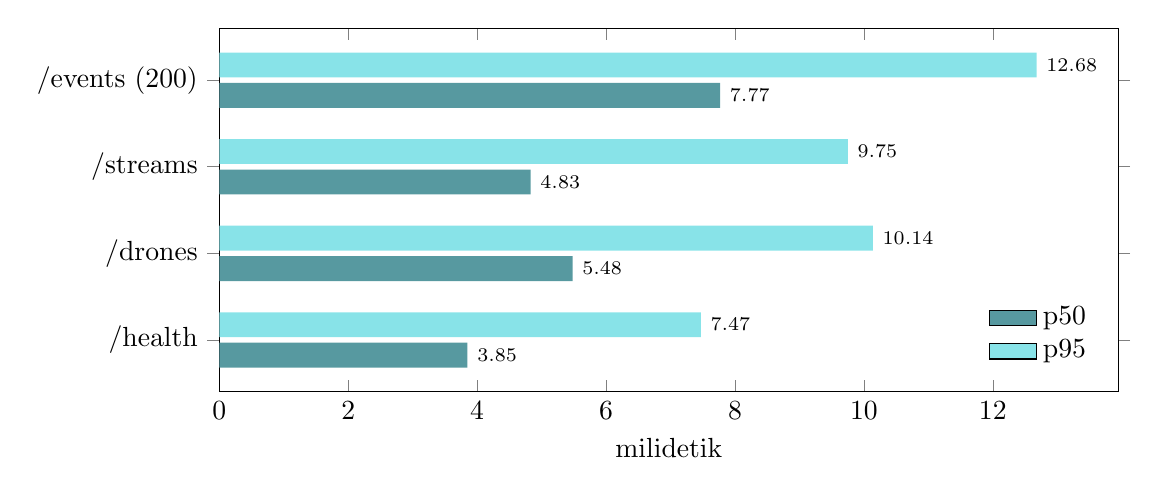
\begin{tikzpicture}
\begin{axis}[xbar, area legend, width=13cm, height=6.2cm, bar width=9pt, xmin=0, xlabel={milidetik}, symbolic y coords={/health,/drones,/streams,/events (200)}, ytick=data,
  legend style={at={(0.98,0.05)},anchor=south east,draw=none}, enlarge y limits=0.2, nodes near coords, nodes near coords style={font=\scriptsize}]
\addplot[fill=teal!70,draw=none] coordinates {(3.85,{/health}) (5.48,{/drones}) (4.83,{/streams}) (7.77,{/events (200)})};
\addplot[fill=cyan!60,draw=none] coordinates {(7.47,{/health}) (10.14,{/drones}) (9.75,{/streams}) (12.68,{/events (200)})};
\legend{p50, p95}
\end{axis}
\end{tikzpicture}
\end{center}
Masing-masing 300 permintaan berurutan.

\section{Telemetri armada}
20 bridge tiruan mengirim format Autel pada 10 Hz. Server menerima 2963 pesan; konsol menerima 1487 frame karena hub realtime sengaja menggabungkan data per drone ke laju siaran 5 Hz (\code{GCS\_\allowbreak{}TELEMETRY\_\allowbreak{}BROADCAST\_\allowbreak{}HZ}) agar peta tetap ringan. Tidak ada data yang hilang di server: seluruh pesan diproses untuk deteksi kejadian dan perekaman.

\section{Batasan pengukuran}
\begin{itemize}
\item Model uji ONNX hanya mengukur overhead pipeline (pra-proses, NMS, publikasi). Waktu inferensi YOLO asli bergantung pada ukuran model dan perangkat (CoreML/MPS di M4, CUDA di NVIDIA).
\item Latensi video WebRTC dan kualitas link radio drone tidak diukur di sini.
\end{itemize}

\section{Mengukur ulang di server produksi}
\begin{lstlisting}
cd backend && . .venv/bin/activate
python tests/bench.py --api http://localhost:8080 --password <sandi-admin> \
  --drones 20 --hz 10 --seconds 15 --out bench-m4.json
\end{lstlisting}
Skrip membuat drone sementara \code{bench-00} dst. lalu menghapusnya kembali.

\chapter{Pemecahan masalah}
\begin{longtable}{@{}p{4.6cm}p{10.4cm}@{}}
\toprule
Gejala & Penyebab dan tindakan \\ \midrule
\endhead
Drone tidak muncul terhubung & IP/port di bridge salah, firewall macOS memblokir 8080, atau ID drone di bridge berbeda dengan di konsol (lihat kejadian \emph{drone tidak dikenal} di Log). \\
Tombol aksi abu-abu \emph{Kendali belum diizinkan} & Interlock di aplikasi bridge mati. DJI: nyalakan sebelum START BRIDGE. Autel: nyalakan lalu SAVE. \\
Perintah \emph{timeout} & Bridge tidak menjawab dalam 10 s (misi 30 s): periksa koneksi Wi-Fi RC dan log aplikasi bridge. \\
DJI menolak \emph{Aktifkan motor} & Perilaku benar: MSDK v5 tidak punya arm terpisah. \\
Lepas landas Autel ditolak & GPS belum valid, kalibrasi kompas/IMU diminta, atau drone tidak di darat. Periksa aplikasi Autel. \\
Misi ditolak & Melebihi batas (120 m, 1 km, 10 m/s, 99 titik) atau posisi drone belum diketahui. Pesan menyebut titik yang bermasalah. \\
Stream \emph{Tidak ada siaran} & Jalur RTMP di perangkat berbeda dengan yang terdaftar, atau port 1935 terblokir. \\
Video hitam di konsol & WebRTC: isi \code{LAN\_IP}, buka UDP 8189; dari luar LAN gunakan VPN. \\
\code{worker: null} di /health & Worker mati atau NATS tak terjangkau: \code{pm2 logs gcs-worker}. \\
Model gagal dimuat & Format tidak cocok dengan worker (CoreML hanya macOS), file rusak, atau paket \code{ultralytics} belum terpasang. \\
Caption tidak muncul & \code{ollama pull moondream}; caption hanya berjalan di mode fokus. \\
STT 503 & faster-whisper belum terpasang di server; konsol memakai STT browser. \\
\bottomrule
\end{longtable}

\chapter{Fitur saat ini dan rencana}
\section{Tersedia di versi 0.3.0}

\noindent\begin{tabularx}{\linewidth}{@{}l X@{}}
\toprule
Area & Fitur \\ \midrule
Armada & Telemetri DJI M4T dan Autel EVO II V3, status link, kejadian lepas landas/mendarat/baterai/RC, rekaman penerbangan dan riwayat jejak. \\
Kendali & Lepas landas, mendarat, RTH, tahan, terbang ke titik, misi waypoint (DJI KMZ, Autel), arm/disarm (Autel), dengan interlock dan batas keselamatan. \\
Video & RTMP/RTSP/HLS/SRT masuk, WebRTC keluar, kamera tetap/CCTV, pemilih lensa DJI. \\
AI & YOLO multi-model, hitungan grup, video beranotasi, caption Moondream dengan terjemahan, tanya-jawab visual, STT. \\
Demo & Drone simulasi dengan misi dan drop payload lengkap. \\
Platform & Web dan desktop Tauri, mode simulasi tanpa server, peran pengguna, log audit, deploy lokal. \\
\bottomrule
\end{tabularx}

\section{Rencana}

\noindent\begin{tabularx}{\linewidth}{@{}l X@{}}
\toprule
Tahap & Fitur \\ \midrule
Berikutnya & Payload drop nyata (DJI PSDK), MAVLink untuk PX4/ArduPilot, telemetri LITO X1 dan SIYI, video jarak jauh lewat TURN/VPN. \\
Lanjutan & Pengenalan wajah, pemetaan 3D, peta luring, integrasi CCTV ONVIF, OpenIPC/WFB-ng. \\
\bottomrule
\end{tabularx}


\appendix
\chapter{Protokol bridge}\label{lamp:protokol}
\section{Endpoint}

\noindent\begin{tabularx}{\linewidth}{@{}l X@{}}
\toprule
URL & Kegunaan \\ \midrule
\code{ws:\allowbreak{}/\allowbreak{}/\allowbreak{}<server>:\allowbreak{}8080/\allowbreak{}telemetry/\allowbreak{}<id>} & Bridge DJI (ID di jalur) \\
\code{ws:\allowbreak{}/\allowbreak{}/\allowbreak{}<server>:\allowbreak{}8080/\allowbreak{}ws/\allowbreak{}drone} & Bridge Autel/generik (\code{droneId} di setiap pesan) \\
\code{ws:\allowbreak{}/\allowbreak{}/\allowbreak{}<server>:\allowbreak{}8080/\allowbreak{}bridge/\allowbreak{}<id>} & Bridge generik dengan ID tetap \\
\bottomrule
\end{tabularx}

Tambahkan \code{?token=\allowbreak{}<GCS\_\allowbreak{}BRIDGE\_\allowbreak{}TOKEN>} bila token diaktifkan.
\section{Pesan}
\begin{lstlisting}
bridge → server  {"type":"hello","droneId":"evo2-v3-001","vendor":"autel",
                  "capabilities":["telemetry","commands","mission"]}
server → bridge  {"type":"command","id":"8f2a…","command":{"type":"takeoff","altM":10}}
server → bridge  {"type":"mission","id":"11b0…","plan":{"name":"Uji","takeoffAltM":20,
                  "endAction":"rtl","waypoints":[{"lat":-6.2,"lon":106.84,"altM":30,
                  "speedMs":3,"holdS":0,"action":"none"}]}}
bridge → server  {"type":"ack","droneId":"evo2-v3-001","id":"8f2a…","accepted":true,
                  "message":"Lepas landas (EVO II naik ±1,2 m lalu hover)"}
bridge → server  {"type":"event","droneId":"evo2-v3-001","severity":"info",
                  "message":"Titik 2/3 tercapai"}
\end{lstlisting}
Permintaan dan jawaban dicocokkan lewat field \code{id}. Batas waktu jawaban: 10 s untuk perintah, 30 s untuk misi.
\section{Telemetri}
DJI (tanpa \code{type}, 10 Hz): \code{pos\{lat,lon,alt\}}, \code{att\{pitch,roll,yaw\}}, \code{vel\{x,y,z\}} (NED), \code{heading}, \code{flying}, \code{sats}, \code{battery}, \code{mode}, \code{motors}, \code{home\{lat,lon\}}, \code{ts}.

Autel (\code{\{"type":\allowbreak{}"telemetry","droneId",.\allowbreak{}.\allowbreak{}.\allowbreak{},"data":\allowbreak{}\{.\allowbreak{}.\allowbreak{}.\allowbreak{}\}\}}, 5 Hz): \code{latitude}, \code{longitude}, \code{relativeAltitude}, \code{roll}, \code{pitch}, \code{yaw}, \code{groundSpeed}, \code{velocityZ}, \code{satelliteCount}, \code{gpsFixType}, \code{batteryPercentage}, \code{flightMode}, \code{homeLatitude}, \code{homeLongitude}, \code{rcSignalLost}, \code{connected}, dan lainnya.
\section{Jenis perintah}
\code{arm}, \code{disarm}, \code{takeoff\{altM\}}, \code{land}, \code{rtl}, \code{hold}, \code{set-mode\{mode\}}, \code{goto\{lat,lon,altM\}}, \code{mission-start}, \code{mission-pause}, \code{payload-release}, \code{set-lens\{lens:\allowbreak{} rgb|thermal|split\}}.

\chapter{Referensi}
\section{Variabel lingkungan API}
\begin{longtable}{@{}p{7.2cm}p{7.8cm}@{}}
\toprule Variabel & Bawaan \\ \midrule \endhead
\code{GCS\_HOST} & \code{"0.0.0.0"} \\
\code{GCS\_PORT} & \code{8080} \\
\code{GCS\_LOG\_LEVEL} & \code{"info"} \\
\code{GCS\_\allowbreak{}DATABASE\_\allowbreak{}URL} & \code{"postgresql:\allowbreak{}/\allowbreak{}/\allowbreak{}gcs:\allowbreak{}gcs@localhost:\allowbreak{}5432/\allowbreak{}gcs} \\
\code{GCS\_NATS\_URL} & \code{"nats:\allowbreak{}/\allowbreak{}/\allowbreak{}localhost:\allowbreak{}4222"} \\
\code{GCS\_\allowbreak{}JWT\_\allowbreak{}SECRET} & \code{""} \\
\code{GCS\_\allowbreak{}JWT\_\allowbreak{}TTL\_\allowbreak{}HOURS} & \code{12} \\
\code{GCS\_\allowbreak{}ADMIN\_\allowbreak{}USERNAME} & \code{"admin"} \\
\code{GCS\_\allowbreak{}ADMIN\_\allowbreak{}PASSWORD} & \code{""} \\
\code{GCS\_\allowbreak{}ADMIN\_\allowbreak{}DISPLAY\_\allowbreak{}NAME} & \code{"Administrator"} \\
\code{GCS\_\allowbreak{}CORS\_\allowbreak{}ORIGINS} & \code{(daftar)} \\
\code{GCS\_\allowbreak{}BRIDGE\_\allowbreak{}TOKEN} & \code{""} \\
\code{GCS\_\allowbreak{}DJI\_\allowbreak{}DEFAULT\_\allowbreak{}DRONE\_\allowbreak{}ID} & \code{"m4t-001"} \\
\code{GCS\_\allowbreak{}AUTEL\_\allowbreak{}ATTITUDE\_\allowbreak{}UNIT} & \code{"deg"} \\
\code{GCS\_\allowbreak{}AUTEL\_\allowbreak{}VZ\_\allowbreak{}DOWN\_\allowbreak{}POSITIVE} & \code{True} \\
\code{GCS\_\allowbreak{}TELEMETRY\_\allowbreak{}BROADCAST\_\allowbreak{}HZ} & \code{5.0} \\
\code{GCS\_\allowbreak{}MEDIAMTX\_\allowbreak{}API\_\allowbreak{}URL} & \code{"http:\allowbreak{}/\allowbreak{}/\allowbreak{}localhost:\allowbreak{}9997"} \\
\code{GCS\_\allowbreak{}MEDIAMTX\_\allowbreak{}RTSP\_\allowbreak{}URL} & \code{"rtsp:\allowbreak{}/\allowbreak{}/\allowbreak{}localhost:\allowbreak{}8554"} \\
\code{GCS\_\allowbreak{}MEDIAMTX\_\allowbreak{}WEBRTC\_\allowbreak{}PUBLIC\_\allowbreak{}URL} & \code{"http:\allowbreak{}/\allowbreak{}/\allowbreak{}localhost:\allowbreak{}8889"} \\
\code{GCS\_\allowbreak{}MEDIAMTX\_\allowbreak{}HLS\_\allowbreak{}PUBLIC\_\allowbreak{}URL} & \code{"http:\allowbreak{}/\allowbreak{}/\allowbreak{}localhost:\allowbreak{}8888"} \\
\code{GCS\_\allowbreak{}MEDIAMTX\_\allowbreak{}LOCAL\_\allowbreak{}HOSTS} & \code{(daftar)} \\
\code{GCS\_\allowbreak{}MODELS\_\allowbreak{}DIR} & \code{"data/models"} \\
\code{GCS\_\allowbreak{}MODEL\_\allowbreak{}MAX\_\allowbreak{}BYTES} & \code{1024 * 1024 * 1024} \\
\code{GCS\_\allowbreak{}MODEL\_\allowbreak{}LOAD\_\allowbreak{}TIMEOUT\_\allowbreak{}S} & \code{180.0} \\
\code{GCS\_\allowbreak{}OLLAMA\_\allowbreak{}URL} & \code{"http:\allowbreak{}/\allowbreak{}/\allowbreak{}localhost:\allowbreak{}11434"} \\
\code{GCS\_VLM\_MODEL} & \code{"moondream"} \\
\code{GCS\_\allowbreak{}TRANSLATE\_\allowbreak{}MODEL} & \code{""} \\
\code{GCS\_\allowbreak{}VLM\_\allowbreak{}TIMEOUT\_\allowbreak{}S} & \code{120.0} \\
\code{GCS\_\allowbreak{}STT\_\allowbreak{}ENGINE} & \code{"faster-whisper"} \\
\code{GCS\_STT\_MODEL} & \code{"small"} \\
\code{GCS\_\allowbreak{}STT\_\allowbreak{}DEVICE} & \code{"cpu"} \\
\code{GCS\_\allowbreak{}STT\_\allowbreak{}COMPUTE\_\allowbreak{}TYPE} & \code{"int8"} \\
\code{GCS\_\allowbreak{}DEMO\_\allowbreak{}ENABLED} & \code{True} \\
\code{GCS\_\allowbreak{}SEED\_\allowbreak{}DEMO\_\allowbreak{}DRONE} & \code{True} \\
\code{GCS\_\allowbreak{}DEMO\_\allowbreak{}BASE\_\allowbreak{}LAT} & \code{-6.2088} \\
\code{GCS\_\allowbreak{}DEMO\_\allowbreak{}BASE\_\allowbreak{}LON} & \code{106.8456} \\
\code{GCS\_\allowbreak{}SIM\_\allowbreak{}TIME\_\allowbreak{}SCALE} & \code{1.0} \\
\bottomrule\end{longtable}
\section{Variabel lingkungan worker}
\begin{longtable}{@{}p{7.2cm}p{7.8cm}@{}}
\toprule Variabel & Bawaan \\ \midrule \endhead
\code{GCS\_\allowbreak{}WORKER\_\allowbreak{}NATS\_\allowbreak{}URL} & \code{nats:\allowbreak{}/\allowbreak{}/\allowbreak{}localhost:\allowbreak{}4222} \\
\code{GCS\_\allowbreak{}WORKER\_\allowbreak{}MODELS\_\allowbreak{}DIR} & \code{data/models} \\
\code{GCS\_\allowbreak{}WORKER\_\allowbreak{}DETECTOR\_\allowbreak{}BACKEND} & \code{auto | ultralytics | onnxruntime} \\
\code{GCS\_\allowbreak{}WORKER\_\allowbreak{}ANNOTATED\_\allowbreak{}OUTPUT} & \code{true} \\
\code{GCS\_\allowbreak{}WORKER\_\allowbreak{}ENCODER} & \code{libx264 | h264\_\allowbreak{}videotoolbox | h264\_\allowbreak{}nvenc} \\
\code{GCS\_\allowbreak{}WORKER\_\allowbreak{}OUTPUT\_\allowbreak{}MAX\_\allowbreak{}WIDTH} & \code{1280} \\
\code{GCS\_\allowbreak{}WORKER\_\allowbreak{}OUTPUT\_\allowbreak{}FPS\_\allowbreak{}CAP} & \code{25} \\
\code{GCS\_\allowbreak{}WORKER\_\allowbreak{}DETECTION\_\allowbreak{}HZ} & \code{5} \\
\code{GCS\_\allowbreak{}WORKER\_\allowbreak{}OLLAMA\_\allowbreak{}URL} & \code{http:\allowbreak{}/\allowbreak{}/\allowbreak{}localhost:\allowbreak{}11434} \\
\code{GCS\_\allowbreak{}WORKER\_\allowbreak{}PROMPTS\_\allowbreak{}FILE} & \code{prompts.\allowbreak{}default.\allowbreak{}toml} \\
\bottomrule\end{longtable}
\section{Endpoint API}
Semua endpoint kecuali \code{/auth/login}, \code{/health}, dan endpoint bridge memerlukan header \code{Authorization:\allowbreak{} Bearer <token>} (WebSocket/SSE: \code{?access\_token=}).
\begin{longtable}{@{}p{2cm}p{13cm}@{}}
\toprule Metode & Jalur \\ \midrule \endhead
GET & \code{/streams} \\
PUT & \code{/\allowbreak{}streams/\allowbreak{}\{stream\_\allowbreak{}id\}/\allowbreak{}model} \\
PUT & \code{/\allowbreak{}streams/\allowbreak{}\{stream\_\allowbreak{}id\}/\allowbreak{}models} \\
POST & \code{/streams/focus} \\
GET & \code{/\allowbreak{}streams/\allowbreak{}\{stream\_\allowbreak{}id\}/\allowbreak{}detections/\allowbreak{}latest} \\
GET & \code{/\allowbreak{}streams/\allowbreak{}\{stream\_\allowbreak{}id\}/\allowbreak{}captions} \\
GET & \code{/models} \\
POST & \code{/models} \\
PATCH & \code{/\allowbreak{}models/\allowbreak{}\{model\_\allowbreak{}id\}} \\
DELETE & \code{/\allowbreak{}models/\allowbreak{}\{model\_\allowbreak{}id\}} \\
POST & \code{/\allowbreak{}models/\allowbreak{}\{model\_\allowbreak{}id\}/\allowbreak{}load} \\
POST & \code{/\allowbreak{}models/\allowbreak{}\{model\_\allowbreak{}id\}/\allowbreak{}unload} \\
POST & \code{/vlm/ask} \\
POST & \code{/stt/transcribe} \\
POST & \code{/auth/login} \\
GET & \code{/auth/me} \\
POST & \code{/\allowbreak{}auth/\allowbreak{}change-password} \\
POST & \code{/auth/logout} \\
GET & \code{/drones} \\
POST & \code{/drones} \\
POST & \code{/\allowbreak{}drones/\allowbreak{}test-link} \\
GET & \code{/\allowbreak{}drones/\allowbreak{}\{drone\_\allowbreak{}id\}} \\
PUT & \code{/\allowbreak{}drones/\allowbreak{}\{drone\_\allowbreak{}id\}} \\
DELETE & \code{/\allowbreak{}drones/\allowbreak{}\{drone\_\allowbreak{}id\}} \\
GET & \code{/\allowbreak{}drones/\allowbreak{}\{drone\_\allowbreak{}id\}/\allowbreak{}flights} \\
POST & \code{/\allowbreak{}drones/\allowbreak{}\{drone\_\allowbreak{}id\}/\allowbreak{}commands} \\
POST & \code{/\allowbreak{}drones/\allowbreak{}\{drone\_\allowbreak{}id\}/\allowbreak{}mission} \\
GET & \code{/cameras} \\
POST & \code{/cameras} \\
PUT & \code{/\allowbreak{}cameras/\allowbreak{}\{camera\_\allowbreak{}id\}} \\
DELETE & \code{/\allowbreak{}cameras/\allowbreak{}\{camera\_\allowbreak{}id\}} \\
GET & \code{/missions} \\
GET & \code{/\allowbreak{}missions/\allowbreak{}\{mission\_\allowbreak{}id\}} \\
POST & \code{/missions} \\
PUT & \code{/\allowbreak{}missions/\allowbreak{}\{mission\_\allowbreak{}id\}} \\
DELETE & \code{/\allowbreak{}missions/\allowbreak{}\{mission\_\allowbreak{}id\}} \\
GET & \code{/drops} \\
POST & \code{/drops} \\
PUT & \code{/\allowbreak{}drops/\allowbreak{}\{drop\_\allowbreak{}id\}} \\
DELETE & \code{/\allowbreak{}drops/\allowbreak{}\{drop\_\allowbreak{}id\}} \\
POST & \code{/\allowbreak{}drops/\allowbreak{}\{drop\_\allowbreak{}id\}/\allowbreak{}execute} \\
POST & \code{/\allowbreak{}drops/\allowbreak{}\{drop\_\allowbreak{}id\}/\allowbreak{}cancel} \\
GET & \code{/events} \\
GET & \code{/health} \\
WS & \code{/ws/realtime} \\
WS & \code{/ws/drone} \\
WS & \code{/\allowbreak{}bridge/\allowbreak{}\{drone\_\allowbreak{}id\}} \\
WS & \code{/telemetry} \\
WS & \code{/\allowbreak{}telemetry/\allowbreak{}\{drone\_\allowbreak{}id\}} \\
\bottomrule\end{longtable}
\section{CLI administrasi}
\begin{lstlisting}
gcs-admin create-user --username <u> --display-name <nama> \
    --role admin|operator|observer [--unit <satuan>]
gcs-admin set-password --username <u>
\end{lstlisting}

\end{document}
